\clearpage
\section{Umsetzung}
\subsection{Benutzerführung}
Die Applikation wurde so als Konsolenapplikation angelegt, dass alle Module auch einzeln verwendet werden können. Für Enduser wurde jedoch im \lstinline$starter.py$ ein Konsolen-gesteuerter Workflow implementiert.

\begin{enumerate}
	\item Titel für die Suche muss eingegeben werden
	\item Der Benutzer wird gefragt, ob er bereits vorhandene Twitterdaten analysieren will oder ob er neue Twitterdaten über das API herunterladen möchte.
	\begin{enumerate}
		\item Wenn der Benutzer neue Twitterdaten laden möchte wird er nach Schlüsselwörtern gefragt
		\item Dem Benutzer werden die eingegebenen Schlüsselwörter nochmals angezeigt und er muss bestätigen damit das API angestossen wird
		\item Die Daten werden heruntergeladen und im File \lstinline$keyword1_keyword2_...keywordn_raw_search_timestamp.txt$ abgelegt. Der Filepfad wird zurückgegeben.
	\end{enumerate}
	\item Wenn der Benutzer vorhandene Twitterdaten analysieren möchte, muss er den Pfad zum Twitterdatenfile angeben
	\item Der Benutzer bestätigt, dass er die Twitter Datenanalyse für die gegebenen Tweets starten möchte
	\item Das Programm analysiert die Daten, erstellt die Plots und ein Logfile mit Resultaten
\end{enumerate}

Live sieht dies wie in Abbildung \ref{fig:benutzerfuehrung} aus.

\begin{figure}[h]
  \centering
  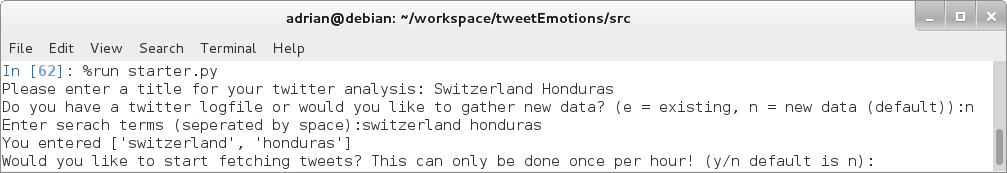
\includegraphics[width=0.8\textwidth]{images/benutzerfuehrung.png}
  \caption[Benutzerführung]{Benutzerführung}
  \label{fig:benutzerfuehrung}
\end{figure}

\subsubsection{Verwendete bzw. Eingebundene Ressourcen}
\begin{table}[H]
\begin{center}
\begin{tabular}{|l|l|}
	\hline
	\lstinline$starter.py$ & Enthält den Code der Benutzerführung \\ \hline
	\lstinline$gather_twitterdata.py$ & Enthält sowohl die Benutzerführung als auch die \\
	& Methoden zum herunterladen der Tweets \\ \hline
	\lstinline$analyse_twitterdata.py$ & Wird mit MPI angestossen um die Daten zu analysieren \\ \hline
\end{tabular}
\caption{Verwendete Ressourcen: Benutzerführung}
\end{center}
\end{table}


\subsection{Twitterdaten Sammeln}
Wie bereits im Kapitel \ref{subsec:grundlagentwitter} beschrieben wurde, zum Herunterladen der Tweets das Package TwitterSearch von Christian Koepp\cite{twittersearch} verwendet.

Im File \lstinline$gather_twitterdata.py$ werden - geführt - Twitterdaten heruntergeladen. Das heisst, der Benutzer wird nach Schlüsselwörtern gefragt, darauf aufmerksam gemacht, dass nach einem Twitter API Call das Interface für eine Weile blockiert sein wird, er muss bestätigen, dass er den Interface Call wirklich mit den von ihm eingegebenen Parametern anstossen will und zum Schluss wird ihm der Dateiname des Twitter Logs angezeigt.

Das Schreiben der Tweets läuft wie folgt ab:
\begin{enumerate}
	\item Tweet und Benutzer auslesen
	\item Zeilenumbrüche im Tweet durch Leerschläge ersetzten
	\item String im Format \lstinline$user \\t tweet \\n$ zusammensetzen
	\item String ins File schreiben 
\end{enumerate}

Wie im Listing \ref{lst:twitterlogformat} ersichtlich, führt dieser Schreibvorgang zu Files, bei welchen auf jeder Zeile ein Benutzername und ein Tweet steht. Innerhalb jeder Zeile sind Benutzernamen und Tweets mit einem Tabulator voneinander getrennt.

\begin{lstlisting}[showtabs=true, caption={Twitter Logfile Format)}, label={lst:twitterlogformat}]
UrbanRadio254	Do you think Sepp Blatter is too old to lead FIFA? #UrbanKickOff
AlanMcnee1	I am thinking of running as head of FIFA. I'm going tae be the new Sepp Blatter. 'Sepp Bladdered.'
blunt_waves	Sepp #Blatter is as corrupt as most of the rulers we have in #Africa. #FIFA.
\end{lstlisting}

\subsubsection{Verwendete bzw. Eingebundene Ressourcen}
\begin{table}[H]
\begin{center}
\begin{tabular}{|l|l|}
	\hline
	\lstinline$gather_twitterdata.py$ & Enthält sowohl die Benutzerführung als auch die\\
	& Methoden zum herunterladen der Tweets \\ \hline
	\lstinline$TwitterSearch$ & Library zum ansteuern der Twitter API\\ \hline
\end{tabular}
\caption{Verwendete Ressourcen: Twitterdaten Sammeln}
\end{center}
\end{table}

\subsection{Algorithmen zur Erkennung der Gefühlslage in Texten}
\subsubsection{Emoticons}
Als Grundlage für den Emoticon Algorithmus wurden als erstes, wie im Listing \ref{lst:emoticonlisting} ersichtlich, Emoticons von den verschiedenen Quellen \cite{emoticons1}\cite{emoticons2}\cite{emoticons3}\cite{emoticons4} zusammengetragen und in die drei Gruppen positiv, negativ und neutral aufgeteilt.

\begin{lstlisting}[language=Python, caption={Emoticon Arrays}, label={lst:emoticonlisting}]
positive = [u'\u263B', u'\263A', u':)', u':D', u':-D', u':]', u':}', u':o)', u':o]', u':o}', u':-]', u':-)', u':-}', u'=)', u'=]', u'=}', u'=^]', u'=^)', u'=^}', u':B', u':-D', u':-B', u':^D', u':^B', u'=B', u'=^B', u'=^D', u':\'), u':\']', u':\'}', u'<3', u'^.^', u'^-^', u'^_^', u'^^', u':*', u'=*', u':-*', u';)', u';]', u';}', u':-p', u':-P', u':-b', u':^p', u':^P', u':^b', u'=P', u'=p', u'/o/', u':P', u':p', u':b', u'=b', u'=^p', u'=^P', u'=^b', u'\o/']
negative = [u'\u2639',u'D:', u'D=', u'D-:', u'D^:', u'D^=', u':(', u':[', u':{', u':o(', u':o[', u':^(', u':^[', u':^{', u'=^(', u'=^{', u'>=(', u'>=[', u'>={', u'>=(', u'>:-{', u'>:-[', u'>:-(', u'>=^[', u'>:-(', u':-[', u':-(', u'=(', u'=[', u'={', u'=^[', u'>:-=(', u'>=[', u'>=^(', u'=\\', u':\\', u'=/', u'=$', u'o.O', u'O_o', u'Oo', u':$:-{', u'>:-{', u'>=^{', u':o{']
neutral = [u':|', u'=|', u':-|', u'>.<', u'><', u'>_<', u':o', u':0', u'=O', u':@', u'=@', u':^o', u':^@', u'-.-', u'-_-', u':x', u'=X', u':-x', u':-@', u':-#', u':^x']
\end{lstlisting}

Um einen Tweet zu analysieren, wird nun mithilfe der Python Methode \lstinline$string.count(substring)$ gezählt wie viele positive, negative und neutrale Emoticons im Tweet vorkommen. Der Rückgabewert bestimmt sich dann wie folgt:

\begin{itemize}
	\item positive - wenn mehr positive als negative Emoticons vorkommen
	\item negative - wenn mehr negative als positive Emoticons vorkommen
	\item neutral - wenn gleich viele positive und negative Emoticons vorkommen oder nur neutrale Emoticons vorhanden sind
	\item unsure - wenn keine Emoticons gefunden wurden
\end{itemize} 

Umgesetzt wurde das Ganze im File \lstinline$emoticon_algorithm.py$.

\subsubsection{SASA}
Die Anwendung des SailAil Sentiment Analyzer war denkbar einfach:

\begin{lstlisting}[language=Python, caption={SASA Classifier}, label={lst:sasaexmaple}]
from sasa.classifier import Classifier
c = Classifier()
classification = c.classifyFromText(tweet) #classification[0] = unicode "neutral", "negative", "positive", "unsure", classification[1] = score
\end{lstlisting}
\subsubsection{Text Preprocessing}
\label{subsubsec:textpreprocessing}
Für die selber implementierten lexikalischen Algorithmen und den eigenen naiven Bayes Ansatz wurden Methoden zur Textvorbereitung umgesetzt. Die Methode \lstinline$preprocessTweet$ ersetzt alle Satzzeichen durch Leerschläge, mehrfache Leerschläge durch einfache, Grossbuchstaben mit den entsprechenden Kleinen und erstellt schliesslich eine Python \lstinline$List$ mit den einzelnen Wörtern.

Die Methode \lstinline$getWordCombinations$ wurde bei den lexikalischen Algorithmen verwendet, um möglichst viele verwendete Ausdrücke (\flqq Wort-Kombinationen\frqq), wie zum Beispiel \flqq monday morning\frqq zu finden.  Die Methode erstellt alle Wort-Kombinationen unter Beachtung der Reihenfolge der Wörter in der Eingabe. Zur Veranschaulichung wird im Listing \ref{lst:preprocessing} die Funktionsweise der Preprocessing Methoden an einem Beispiel gezeigt.

\begin{lstlisting}[language=Python, caption={Text Preprocessing}, label={lst:preprocessing}]
In [11]: words = preprocessing.preprocessTweet("Everyone loves monday mornings!") 
In [12]: print words
['everyone', 'loves', 'monday', 'mornings']

In [13]: wordcombos = preprocessing.getWordCombinations(words, " ")

In [14]: print wordcombos
['everyone', 'everyone loves', 'everyone loves monday', 'everyone loves monday mornings', 'loves', 'loves monday', 'loves monday mornings', 'monday',  'monday mornings', 'mornings']
\end{lstlisting} 

\subsubsection{SentiWordNet}
Der SentiWordNet Algorithmus wurde als Python Klasse implementiert. Im Konstruktor wird das Wörterbuch aus dem File eingelesen und in ein Python Dictionary verwandelt. Die Vorgehensweise ist dabei an die Java-Beispielimplementation von Petter Törnberg \cite{sentiwordnetjava} angelehnt. Grob funktioniert es wie folgt:

\begin{enumerate}
	\item Das Wörterbuch (Textfile) wird eingelesen und nach Zeilen aufgeteilt. Die folgenden Aktionen werden für jede Zeile ausgeführt.
	\item Wenn ein \# am Anfang der Zeile steht wird sie ignoriert.
	\item Die Zeile wird nach Tabulatoren aufgesplittet.
	\item Wenn die Zeile nicht aus 6 Elementen besteht, wird eine Fehlermeldung ausgegeben.
	\item Der Synset-Score der Zeile wird berechnet ($positiveScore - negativeScore$).
	\item Das Synset wird aufgesplittet und jedes Wort des Synsets wird zusammen mit dem Rank in ein temporäres \lstinline$Dictionary$ geschrieben (\lstinline$tmpDict[wort][rank] = synSetScore$).
	\item Der SentiNetScore für jedes Wort entspricht dem gewichteten Durchschnitt der SentiScores aller Vorkommnisse dieses Wortes und wird wie folgt berechnet: $\frac{\frac{1}{2}\cdot Rank_1 + \frac{1}{3} \cdot Rank_2 + ... + \frac{1}{n} \cdot Rank_n}{1+\frac{1}{2}+\frac{1}{3}+...+\frac{1}{n}}$.
	\item Im finalen \lstinline$Dictionary$ werden jeweils das Wort und der entsprechende SentiNetScore abgelegt.
\end{enumerate}

Mit dem so erstellten Dictionary kann man einfach den SentiNetScore für Wörter und Ausdrücke auslesen. (\lstinline$sentiNetScore = ditct[ausdruck]$). Der Methode \lstinline$getTweetScore$ kann ein Tweet übergeben werden. Dieser wird zuerst vorverarbeitet (Sprich es werden alle Wort-Kombinationen generiert. Siehe Kapitel \ref{subsubsec:textpreprocessing}). Nun wird für jeden Ausdruck in der generierten Liste der SentiWordNet Score gesucht und schlussendlich wird der Durchschnitt der gefunden Scores wie folgt berechnet und zurückgegeben.
\begin{equation}
avg = \sum_{i=1}^{n} \frac{sentiWordNetScore(expression_i)}{n}
\end{equation}
Implementiert ist das Beschriebene im Python File \lstinline$sentiwordnet.py$.

\subsubsection{SenticNet}
Auch der SenticNet Algorithmus wurde als Python Klasse implementiert. Im Konstruktor wird in diesem Falle das XML File geparst. Das im SenticNet alle Wörter nur einmal vorkommen, werden diese direkt in ein \lstinline$Dictionary$ eingelesen. Der SenticNet Score besteht jeweils aus 5 Werten und ist in einer kleinen Klasse \lstinline$SenticScore$ abgebildet. Diese Klasse kann unter anderem geplottet werden (\lstinline$SenticScore.plot()$) und die SenticNet Polarity gemäss Formel \ref{equ:senticpolarity} berechnen.

\begin{equation}
\label{equ:senticpolarity}
p = \sum_{i=1}^{N} \frac{Plsnt(c_i)+|Attnt(c_i)|-|Snst(c_i)|+Aptit(c_i)}{3N}
\end{equation}

Das Verarbeiten der Tweets läuft dann äquivalent zur Verarbeitung von Tweets mit dem SentiWordNet Algorithmus ab. Anstelle des Floats, welchem der SentiWordNet Score entspricht, werden hier einfach die SentiScore Objekte aufsummiert und daraus wird dann der Durchschnitt berechnet. 

Die Implementation dieses Algorithmus befindet sich im File \lstinline$senticnet.py$ 

\subsubsection{NLTK naive Bayes}
Der letzte Implementierte Ansatz unter Verwendung der NLTK eigenen naive Bayes Implementation ist wie bereits im Kapitel \ref{subsubsec:grundlagennaivebayes} beschrieben, stark an den Artikel von Jacob Perkins \cite{nltkbayes} angelehnt. Konkret wurde wiederum eine Klasse implementiert, in deren Konstruktor alles nötige initialisiert wird. In diesem Falle wird im Konstruktor der naive Bayes Algorithmus mithilfe des NLTK Movie Review Korpus trainiert.

Sowohl das Trainieren, als auch das Klassifizieren sind wie in Listing \ref{lst:naivebayes} aufgezeigt denkbar unspektakulär:

\begin{lstlisting}[language=Python, caption={Naive Bayes Training \& Klassifizieren}, label={lst:naivebayes}]
from nltk.classify import NaiveBayesClassifier
from nltk.corpus import movie_reviews

class NLTKTweetClassifier:
	def word_feats(self, words):
	    return dict([(word, True) for word in words])

	def classifyTweet(self, tweet):
		words = preprocessTweet(tweet)
		return self.classifier.classify(self.word_feats(words))

	def __init__(self):
		trainfeats = getTrainFeats() #get training set
		self.classifier = NaiveBayesClassifier.train(trainfeats) #training
\end{lstlisting}

Implementiert ist dieser Algorithmus im File \lstinline$nltk_tweet_classifier.py$.

\subsection{Parallelisierung}
Um die Performanz der Berechnungen zu erhöhen, wurde das Analysieren der Tweets mithilfe von MPI parallelisiert. Der Ablauf des parallelisierten Algorithmus ist dabei wie folgt:

\begin{enumerate} 
\item RANK 0: das Config \lstinline$config/config.txt$ mit den Eigabeparametern \lstinline$filename$ (Des Twitter Logfiles) und \lstinline$title$ (Der Analyse) wird eingelesen
\item RANK 0: das Twitterlogfile \lstinline$filename$ wird eingelesen und es wird eine Liste von Tweets erzeugt
\item RANK 0: Die Algorithmen SenticNet und SentiWordNet werden initialisiert
\item ALLE: Die Algorithmen SASA und NLTK werden initialisiert (Die Objekte können nicht über das MPI COMM transferiert werden)
\item ALLE: Die Tweet-List, die SenticNet Instanz und die SentiWordNetInstance werden per Broadcast vom RANK 0 an alle übertragen
\item ALLE: Jedem Prozess werden \lstinline$len(Tweet-List)/AnzahlProzesse$ Tweets zugeteilt
\item ALLE: Jeder Prozess analysiert die ihm zugeteilten Tweets mithilfe der \lstinline$analyseTweet()$ Methode und schreibt das Ergebnis in eine \lstinline$resultList$
\item ALLE: Die resultList wird an den Prozess 0 übermittelt
\item RANK 0: Die Resultat-Listen der einzelnen Prozesse werden zusammengesetzt, zusammengefasst und geplottet 
\end{enumerate}

Während dem ganzen Prozess wird die Zeit, welche für die einzelnen Schritte benötigt wird berechnet und sowohl ausgegeben als auch in einem Logfile abgelegt.

\subsubsection{Verwendete bzw. Eingebundene Ressourcen}
\begin{table}[H]
\begin{center}
\begin{tabular}{|l|l|}
	\hline
	\lstinline$analyse_twitterdata.py$ & Enthält den mit MPI parallelisierten Ablauf\\ \hline
	\lstinline$analyse_tweet.py$ & Enthält sowohl den Code zum analysieren eines Tweets, als auch\\
	& den Code zum zusammenfassen und Plotten der Resultate\\ \hline
	\lstinline$autolabel.py$ & Ein Codesnippet zum Beschriften der Matplotlib Balken\\ \hline
	\lstinline$emoticon_algorithm.py$ & Der verwendete Emoticon Algorithmus\\ \hline
	\lstinline$logger.py$ & Ein sehr einfacher Logger der verwendet wird um die \\
	& Textausgabe in ein File zu schreiben\\ \hline
	\lstinline$nltk_tweet_classifier.py$ & Der verwendete NLTK Classifier\\ \hline
	\lstinline$sasa_tweet_classifier.py$ & Der verwendete SASA Algorithmus\\ \hline
	\lstinline$senticnet.py$ & Der verwendete SenticNet Algorithmus\\ \hline
	\lstinline$sentiwordnet.py$ & Der verwendete SentiWordNet Algorithmus\\ \hline
\end{tabular}
\caption{Verwendete Ressourcen: Parallelisierung}
\end{center}
\end{table}